\documentclass[11pt,a4paper]{article}
\usepackage[T1]{fontenc}
\usepackage[utf8]{inputenc}
\usepackage{mathptmx}          % Times New Roman ile metrik-uyumlu klon (Nimbus Roman)
\usepackage[margin=2.4cm]{geometry}
\usepackage{graphicx}
\usepackage{booktabs}
\usepackage{float}
\usepackage{caption}
\captionsetup{font=small,labelfont=bf}
\renewcommand{\figurename}{Şekil}
\renewcommand{\tablename}{Tablo}
\linespread{1.08}
\setlength{\parindent}{1.2em}
\usepackage[hidelinks]{hyperref}

\graphicspath{{figurler/}}

\begin{document}

\begin{titlepage}
\centering
\vspace*{2cm}
{\large KOCAELİ ÜNİVERSİTESİ\par}
{\large Mühendislik Fakültesi --- Bilgisayar Mühendisliği (İkinci Öğretim)\par}
\vspace{2.5cm}
{\large Pekiştirmeli Öğrenme Dönem Projesi\par}
\vspace{0.8cm}
{\Huge\bfseries GPS'siz Bir Drone'un Kapalı\\[0.3cm] Ortamda PPO ile Keşfi\par}
\vspace{2.5cm}
{\large Berker Yiğit\par}
{\large 220202046\par}
\vfill
{\large Haziran 2026\par}
\end{titlepage}

\section{Giriş}

Bu projede, konumunu bir GPS alıcısından değil yalnızca lidar ve odometri ölçümlerinden çıkaran
bir insansız hava aracının, içinde hareketli engeller bulunan kapalı bir binayı çarpmadan ve
mümkün olduğunca geniş biçimde keşfetmesi hedeflendi. Problem, klasik yol planlamadan farklı olarak,
haritanın önceden bilinmediği ve çevrenin durağan olmadığı bir durumda ortaya çıkıyor; bu nedenle
çözümü, ortamla etkileşerek öğrenen bir pekiştirmeli öğrenme ajanına bıraktım. Algoritma olarak,
sürekli aksiyon uzaylarında kararlı davranışıyla bilinen PPO (Proximal Policy Optimization) seçtim.
Projenin amacı tek bir cümleyle özetlenebilir: ajan, hareketli engellere çarpmadan, binadaki
zemin hücrelerinin (voxel) olabildiğince çoğunu gezmeyi öğrenmeli.

Raporun ilerleyen bölümlerinde önce ortamı ve yöntemi tanıtıyor, ardından projenin iki temel
bulgusunu---çarpışmanın aslında bir gözlem tasarımı problemi olduğunu ve keşif genişliği ile
güvenlik arasında giderilemeyen bir ödünleşim bulunduğunu---deneylerle açıklıyorum. Yaptığım her
parametre değişikliğinin gerekçesini, gözlemlenen sonuçla birlikte veriyorum.

\section{Ortam ve Yöntem}

Çalışma ortamı, on altıya on altı metrelik, tek katlı ve altı odadan oluşan sabit bir binadır.
Odalar iki metrelik kapı boşluklarıyla birbirine bağlanır ve drone her bölüme aynı köşeden, R0
odasından (koordinat $-5,-5$) başlar; bu sayede sonuçlar bölümden bölüme adil biçimde
karşılaştırılabilir. Ortamda üç dairesel engel sabit periyotlarla salınım yaparak hareket eder,
dolayısıyla ajanın yalnızca duvarlardan değil zamanla yer değiştiren engellerden de kaçınması
gerekir.

Ajanın aksiyonu iki boyutludur: ileri/geri doğrusal hız ile dönüş açısal hızı. İrtifa sabit
tutulduğundan dikey hareket yoktur. Gözlem vektörü kırk boyutludur ve otuz iki yöne bölünmüş lidar
demetlerinin yanı sıra yönelimin sinüs/kosinüsünü, anlık hızları, o ana kadar keşfedilen alan oranını,
ziyaret edilen oda sayısını ve en yakın engele olan uzaklığı içerir. Ödülü, toplam getirinin
keşfedilen voxel sayısına yaklaşacağı bir felsefeyle kurdum: her yeni hücre artı bir puan, yeni bir
odaya ilk geçiş büyük bir ödül, bir metreden yakın bir engele yaklaşma küçük bir ceza, fiziksel
çarpışma ise bölümü sonlandıran ağır bir cezadır. Bu sade tasarımın gerekçesi ileride netleşecek
karşılaştırmalarla doğrulandı.

PPO eğitiminde Stable-Baselines3 kütüphanesini kullandım. Politika ağı her biri iki yüz elli altı
nöronlu iki gizli katmandan oluşur; öğrenme oranı doğrusal olarak $3\times10^{-4}$'ten
$1\times10^{-5}$'e azalır, rollout uzunluğu 1024 adım, yığın boyutu 512, dönem sayısı on, indirim
çarpanı $\gamma=0{,}99$, GAE $\lambda=0{,}95$, kırpma aralığı $0{,}2$ ve entropi katsayısı
$0{,}008$'dir. Ödüller \texttt{VecNormalize} ile normalize edilir ve eğitim sekiz paralel ortamda
yürütülür. Bu değerler, aşağıda anlatılan deneylerin tümünde sabit kalan iskeleti oluşturur;
versiyonlar arasında değiştirdiğim şey ödül katsayıları ve eğitim süresi oldu.

Tablo~\ref{tab:param}, projedeki üç önemli sürümün ödül ve eğitim ayarlarını yan yana verir; bu
değerler doğrudan ilgili \texttt{configs/fast\_v4\_*.yaml} dosyalarından alınmıştır.

\begin{table}[H]
\centering
\caption{Önemli sürümlerin yapılandırma değerleri (YAML dosyalarından).}
\label{tab:param}
\small
\begin{tabular}{lccc}
\toprule
Parametre & v4.1 & v4.8 & v4.10 \\
\midrule
\texttt{room\_bonus} (yeni oda ödülü) & 30 & 30 & 30 \\
\texttt{collision\_penalty} (çarpışma cezası) & 10 & 25 & 25 \\
\texttt{far\_voxel\_bonus} (uzak hücre ödülü) & 0 & 1{,}0 & 1{,}0 \\
\texttt{idle\_penalty} / \texttt{idle\_grace} & 0{,}05 / 40 & 0{,}06 / 30 & 0{,}06 / 30 \\
\texttt{lidar\_history} (gözlem karesi) & 2 & 2 & 2 \\
\texttt{ent\_coef} & 0{,}008 & 0{,}008 & 0{,}008 \\
\texttt{total\_timesteps} (eğitim adımı) & 2\,M & 2\,M & 5\,M \\
\bottomrule
\end{tabular}
\end{table}

Başlangıçta ortamı Gazebo ve ROS~2 üzerinde modelledim. Ancak bu kurulum saniyede yaklaşık kırk
adım üretebildiğinden tek bir eğitim saatler sürüyordu. Aynı iki boyutlu ortamı numpy ile, ışın-segment
ve ışın-daire kesişimlerine dayanan bir tarama olarak yeniden yazınca hız saniyede yaklaşık dört bine
çıktı; böylece bir gün içinde çok sayıda denemeyi tamamlayabildim. Gazebo sonuçlarını silmedim,
çünkü aynı ortamın iki ayrı motorda benzer eğilimler göstermesi bulguların güvenilirliğini artırıyor.

\section{Çarpışma: Aslında Bir Gözlem Problemi}

İlk ciddi sonuçları Gazebo'daki sade ödüllü sürümle (v2.0) aldım: yüz bölümlük değerlendirmede
çarpışma oranı yüzde yetmiş, birleşik kapsama yüzde otuz altıydı. Çarpışmayı azaltmak için ödüle
daha akıllı görünen ceza terimleri ekledim; örneğin yalnızca ilerideki engelleri cezalandıran
yön duyarlı bir terim denedim. Sonuç beklediğimin tersi oldu: çarpışma önce yüzde yetmiş dokuza,
yanlardan gelen tehditleri de kapsayan birleşik bir cezada ise yüzde seksen sekize yükseldi. Bu
başarısızlık öğreticiydi, çünkü asıl darboğazın ödül biçimlendirmesinde değil gözlemde olduğunu
gösterdi: ajan engelin yalnızca o anki uzaklığını görüyor, hangi yöne ne hızla geldiğini
göremiyordu.

Çözüm tek bir tasarım değişikliğiyle geldi. Gözleme yalnızca güncel lidar karesini değil ardışık
iki kareyi koyduğumda (\texttt{lidar\_history}~$=2$) ajan iki kare arasındaki farktan engelin
hızını çıkarabildi ve önünden çekilmeyi öğrendi. Çarpışma oranı yüzde seksenlerden yüzde bire
düştü. Aylarca süren ödül ayarının çözemediği problemi, ajana \emph{ne gösterdiğimi} değiştirmek
çözdü. Şekil~\ref{fig:cozum} bu sürümün kapsama ısı haritasını gösterir.

\begin{figure}[H]
\centering
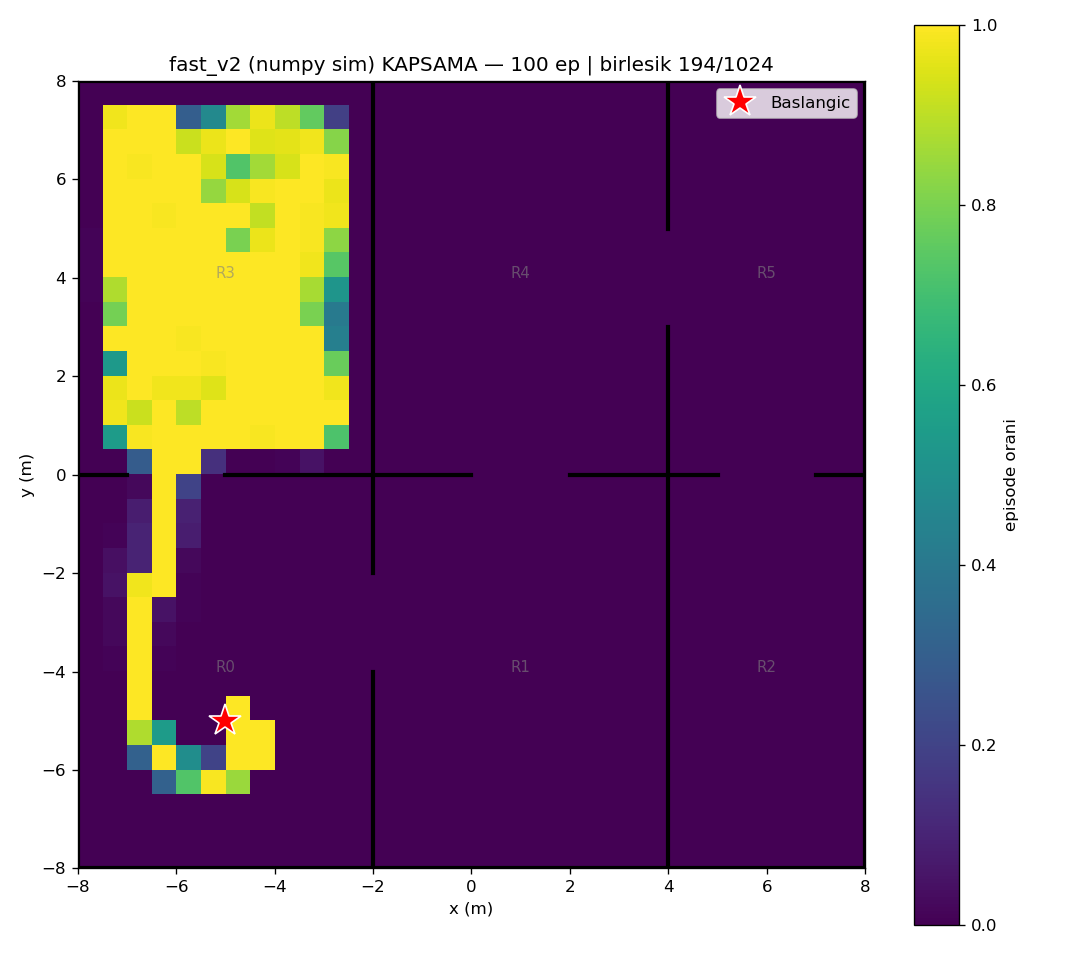
\includegraphics[width=0.6\linewidth]{07_fast_v2_carpisma_cozuldu_kapsama.png}
\caption{Lidar geçmişi eklendikten sonra çarpışmanın çözüldüğü sürümün kapsama haritası. Renk,
yüz bölüm boyunca bir hücrenin ne sıklıkla ziyaret edildiğini gösterir.}
\label{fig:cozum}
\end{figure}

\section{Keşif Genişliği ile Güvenlik Arasındaki Ödünleşim}

Çarpışma çözülünce yeni bir sorun belirdi. Güvenliği önceleyen ajan aşırı temkinli davranıp
yalnızca başlangıca yakın iki odayı tarıyor, risk almamak için uzak odalara hiç gitmiyordu.
Genişliği artırmak için ödül katsayılarını teker teker değiştirip her birinin etkisini ölçtüm.

Önce oda ödülünü on'dan otuza çıkardım. Bu değişiklik güvenliği daha da iyileştirdi ama tek başına
keşfi açmadı, çünkü ajan uzak bir odaya hiç gitmediğinden oranın değerini öğrenemiyordu. Ardından
başlangıçtan uzak hücreleri ek olarak ödüllendiren \texttt{far\_voxel\_bonus} terimini bir'e
çıkardım; bu, ajanı dışarı doğru iterek beş odaya yaymayı başardı, ancak çarpışma yükseldi. Nedeni
açıktı: çarpışma cezası eksi on iken, bir bölümde toplanan keşif ödülü yüz otuzu aşıyordu, yani
ajan için ``keşfet ve sondaki küçük cezayı kabul et'' davranışı kârlıydı.

Bu gözlem, projenin en belirleyici değişikliğine yol açtı. Çarpışma cezasını yirmi beşe
çıkardığımda davranış kökten değişti: keşif tamamlandıktan sonra geriye yalnızca çarpıp ağır ceza
almak ya da bölümü sağ bitirmek kaldığından, ajan ``önce gez, sonra hayatta kal'' stratejisini
benimsedi ve çarpışma oranı yüzde sıfıra indi. Bu sürüm (v4.8) yüz bölümün tamamını çarpmadan
tamamladı ve her bölümde altı odanın beşine ulaştı (Şekil~\ref{fig:guvenli}). Beklemediğim bir
ayrıntı, cezayı otuz yerine yirmi beşte bırakmanın daha iyi sonuç vermesiydi; çok yüksek ceza,
ajanı aşırı tedbirli yapıp ara sıra hatalı kaçınma manevralarına itiyordu. Yani buradaki kazanç,
cezayı sürekli büyütmekte değil, dar bir tatlı noktayı bulmakta yatıyordu.

\begin{figure}[H]
\centering
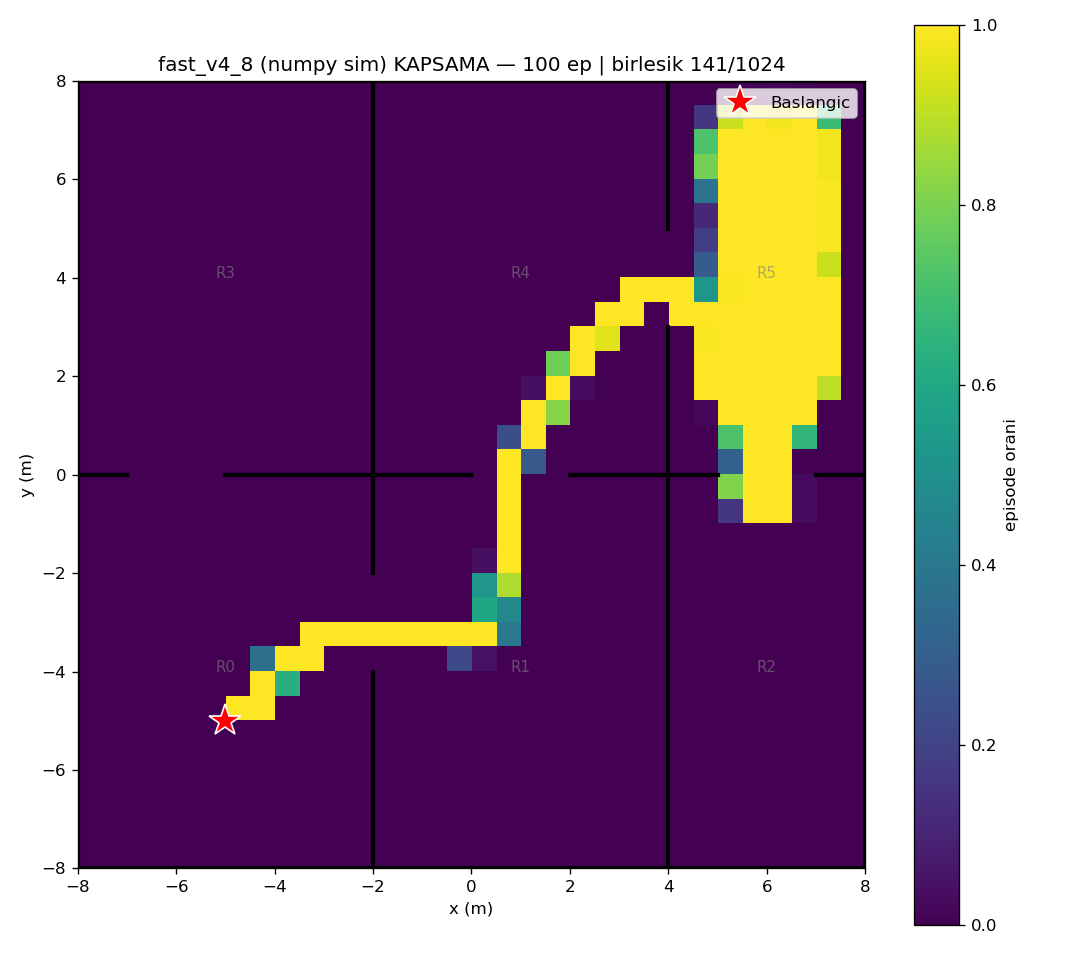
\includegraphics[width=0.6\linewidth]{03_v4_8_GUVENLI_kapsama.png}
\caption{Güvenli sürüm v4.8: yüz bölümde hiç çarpışma yok, beş oda düzenli olarak taranıyor.
Renkli bölgelerin başlangıç köşesinden odalara doğru yayıldığı görülür.}
\label{fig:guvenli}
\end{figure}

Aynı ödülle yalnızca eğitim süresini iki milyon adımdan beş milyona çıkardığımda (v4.10) ilginç bir
sonuç aldım: ortalama kapsanan voxel yüz on yediden iki yüz seksen bire, ulaşılan oda sayısı beşten
altıya çıktı ve birleşik kapsama yüzde kırk dört buçuğa ulaştı; ancak çarpışma oranı yüzde elli
dörde yükseldi (Şekil~\ref{fig:kapsam}). Bunun nedeni, daha uzun eğitimde biriken keşif ödülünün
sabit kalan çarpışma cezasını yeniden bastırmasıdır. Dolayısıyla eğitim süresinin kendisi de bu
ödünleşim üzerinde bir ayar düğmesi gibi davranıyor; ödülü hiç değiştirmeden, yalnızca daha uzun
eğiterek ajanı cesur ama riskli bir uca taşımak mümkün.

\begin{figure}[H]
\centering
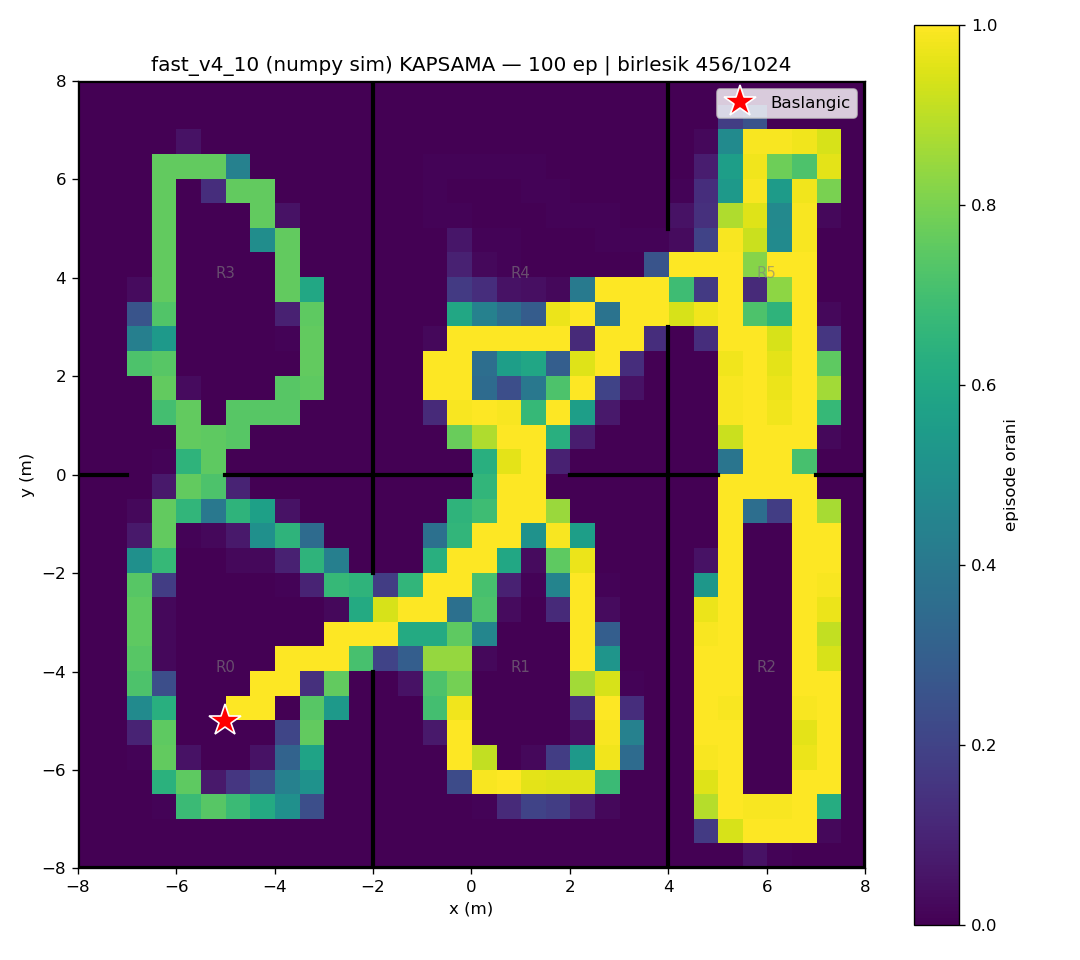
\includegraphics[width=0.6\linewidth]{05_v4_10_KAPSAM_kapsama.png}
\caption{Kapsam sürümü v4.10: aynı ödül, beş milyon adım eğitim. Altı odanın tamamı ve haritanın
neredeyse yarısı kapsanıyor; bedeli yüksek çarpışma oranıdır.}
\label{fig:kapsam}
\end{figure}

Burada dikkat edilmesi gereken bir yanılgıya da değinmek isterim. Çarpışma cezası düşük ve uzak
hücre ödülü kapalı olan erken bir sürüm (v4.1), bölüm başına yüz elli voxel gibi yüksek bir sayı
ve yalnızca yüzde iki çarpışmayla cazip görünüyordu. Oysa bu sürüm hep aynı iki odayı yoğun biçimde
tarıyor, yeni odalara yayılmıyordu; birleşik kapsaması yüzde altıda kalıyordu. Bu örnek, asıl
ödünleşimin ``voxel sayısı ile çarpışma'' değil, ``kaç farklı odaya yayıldığın ile güvenlik''
olduğunu açıkça gösterdi. Yüksek voxel her zaman geniş keşif anlamına gelmiyor.

\section{Sonuç ve Değerlendirme}

Yaptığım on dört deney, ödül biçimlendirmesi, eğitim süresi, önceki modelden ince ayar ve gözlem
zenginliği gibi birbirinden bağımsız dört yolu denememe rağmen aynı sonuca çıktı: bu ortam, bu ödül
ve bu aksiyon uzayında keşif genişliği ile güvenlik aynı anda en üst düzeye çıkarılamıyor.
Şekil~\ref{fig:pareto} bütün sürümleri tek bir grafikte toplar; sol üstte arzu edilen ``hem geniş
hem güvenli'' bölge boş kalır, ulaşılabilir noktalar bir Pareto cephesi çizer. Şekil~\ref{fig:egri}
ise temsili sürümlerin eğitim boyunca ödül, voxel, oda ve bölüm uzunluğu eğrilerini gösterir.

\begin{figure}[H]
\centering
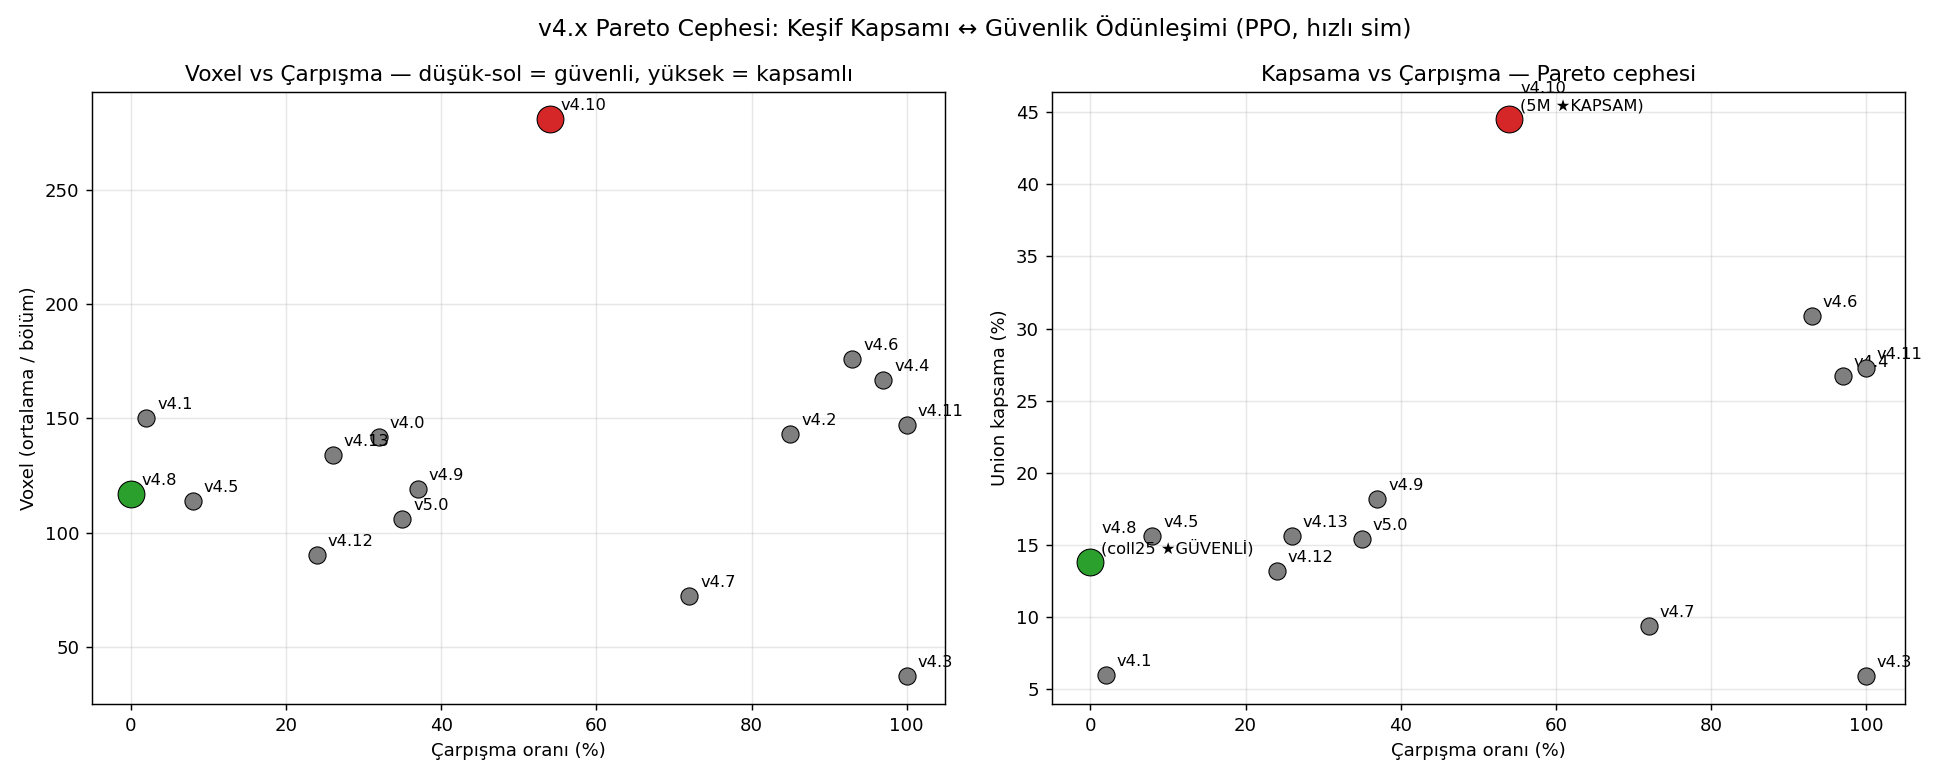
\includegraphics[width=0.92\linewidth]{01_pareto_cephesi.png}
\caption{Tüm sürümlerin kapsama--çarpışma düzlemindeki dağılımı. Yeşil nokta güvenli uç (v4.8),
kırmızı nokta kapsam ucudur (v4.10); ikisinin arasında ``hem yüksek kapsam hem sıfır çarpışma''
noktası yoktur.}
\label{fig:pareto}
\end{figure}

\begin{figure}[H]
\centering
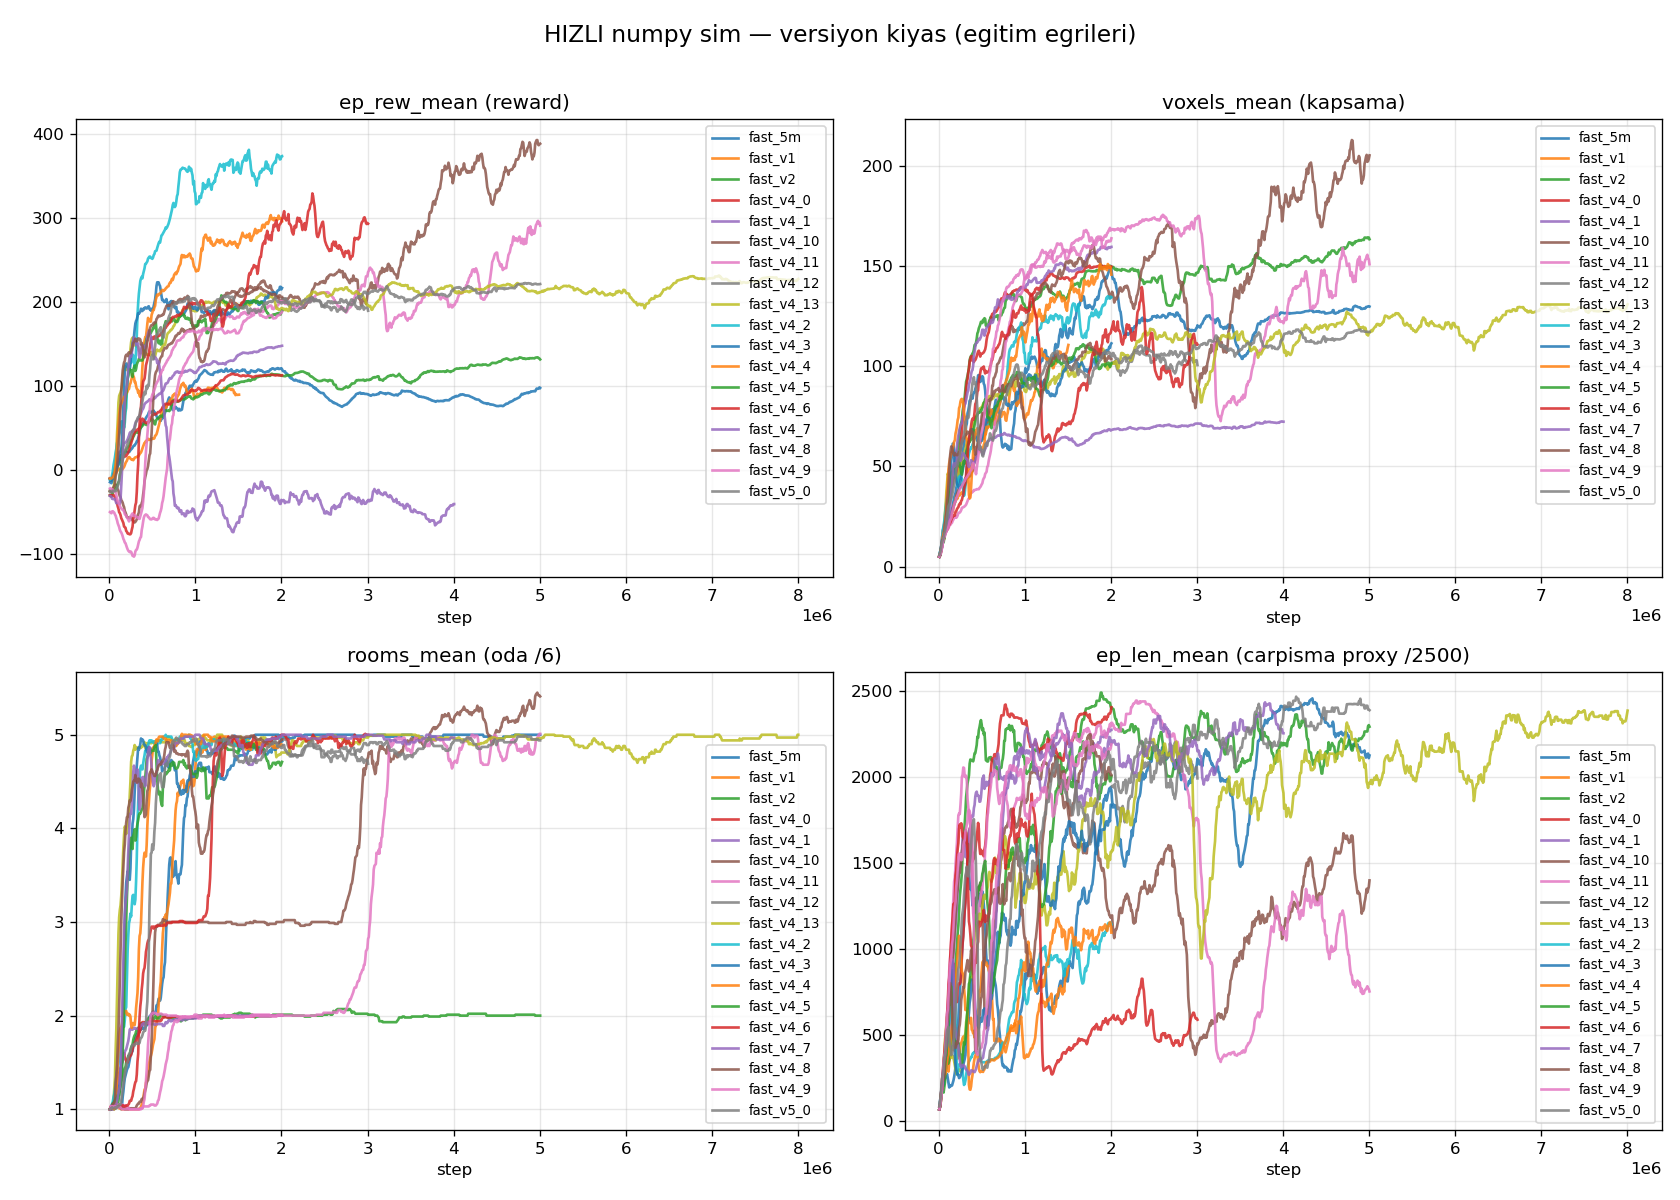
\includegraphics[width=0.95\linewidth]{02_egitim_egrileri_v4_v5.png}
\caption{Temsili sürümlerin eğitim eğrileri: ortalama ödül, kapsanan voxel, ziyaret edilen oda ve
bölüm uzunluğunun adım sayısına göre değişimi.}
\label{fig:egri}
\end{figure}

Sonuç olarak iki politikayı teslim ediyorum. Güvenli sürüm v4.8, ``çarpmadan geniş keşif'' hedefini
gerçekten karşılayan tek çözümdür: yüzde sıfır çarpışmayla altı odanın beşini düzenli olarak gezer
ve görevi her zaman güvenle tamamlar. Kapsam sürümü v4.10 ise modelin kapasite tavanını gösterir;
yeterince uzun eğitildiğinde binanın neredeyse tamamını kapsayabildiğini, ancak bunun güvenlikten
ödün vermeden mümkün olmadığını kanıtlar. Proje hedefi ``çarpışmadan maksimum keşif'' olduğundan
önerdiğim ana sonuç v4.8'dir; v4.10 onu tamamlayan bir üst sınır kanıtı niteliğindedir.

Gazebo ve numpy karşılaştırması da bu sonucu destekledi: yavaş ama gerçekçi Gazebo'da en iyi sürüm
yüzde yetmiş çarpışma ve yüzde otuz altı kapsamada kalırken, hızlı numpy ortamında gözlem tasarımını
düzelttikten sonra çarpışmayı tümüyle ortadan kaldırabildim. İleride bu cepheyi daha iyiye taşımak
için, sabit kare yığını yerine belleğe sahip yinelemeli bir politika (RecurrentPPO) veya engel
hızını kademeli artıran bir müfredat denenebilir; ancak bunlar projenin sabit kıstaslarını
değiştireceğinden, mevcut bulgular bu kıstaslar altında eksiksiz kabul edilmelidir.

\end{document}
